\documentclass[12pt]{report}
\usepackage{setspace}
%\usepackage{subfigure}

\pagestyle{plain}
\usepackage{amssymb,graphicx,color}
\usepackage{amsfonts}
\usepackage{latexsym}
\usepackage{a4wide}
\usepackage{amsmath}
\usepackage[hidelinks]{hyperref}
\usepackage{booktabs}
\usepackage[table]{xcolor}
\usepackage{multirow}
\usepackage{rotating}

% \hypersetup{
%   colorlinks=false,
%   urlcolor=cyan,
%   pdftitle={Overleaf Example},
%   pdfpagemode=FullScreen,
% }

\newtheorem{theorem}{THEOREM}
\newtheorem{lemma}[theorem]{LEMMA}
\newtheorem{corollary}[theorem]{COROLLARY}
\newtheorem{proposition}[theorem]{PROPOSITION}
\newtheorem{remark}[theorem]{REMARK}
\newtheorem{definition}[theorem]{DEFINITION}
\newtheorem{fact}[theorem]{FACT}

\newtheorem{problem}[theorem]{PROBLEM}
\newtheorem{exercise}[theorem]{EXERCISE}
\def \set#1{\{#1\} }
\def\code#1{\texttt{#1}}

\newenvironment{proof}{
PROOF:
\begin{quotation}}{
$\Box$ \end{quotation}}



\newcommand{\nats}{\mbox{\( \mathbb N \)}}
\newcommand{\rat}{\mbox{\(\mathbb Q\)}}
\newcommand{\rats}{\mbox{\(\mathbb Q\)}}
\newcommand{\reals}{\mbox{\(\mathbb R\)}}
\newcommand{\ints}{\mbox{\(\mathbb Z\)}}
\newcommand*\rot{\rotatebox{90}}

%%%%%%%%%%%%%%%%%%%%%%%%%%


\title{  	{ 
\includegraphics[scale=.5]{ucl_logo.png}}\\
{{\Huge Two Little Birds: A Study in Birdsong Binary Classification Problems}}\\
% {\large Optional Subtitle}
}
\date{Submission date: 11 September 2023}
\author{Candidate Number: YPDR0\thanks{
{\bf Disclaimer:}
This report is submitted as part requirement for the MSc Data Science \& Machine
Learning at UCL. It is substantially the result of my own work except where
explicitly indicated in the text. The report may be freely copied and
distributed provided the source is explicitly acknowledged
}
\\ \\
MSc Data Science \& Machine Learning\\ \\
Supervisor: Dr.\ Ifat Yasin}


\begin{document}
 
 \onehalfspacing
\maketitle
\begin{abstract}
Automated or semi-automated birdsong classification forms a key tool in a wide
range of important fields, such as ecological surveying, climate modelling, and
birdwatching for pleasure. With a recent surge in popularity of machine learning
techniques and a wealth of of publicly available datasets, these problems are
increasingly being tackled using state-of-the-art machine learning approaches
with better and better results. This work will focus on investigating and
evaluating popular approaches to birdsong classification problems, as well as
experimenting with recent research into wider audio classification problems and
evaluating them in a birdsong context.

\end{abstract}
\tableofcontents
\setcounter{page}{1}


\chapter{Introduction}\label{cp:intro}
Birds play a crucial role in ecosystems around the world. They form an important
link in the food chain, pollinate plants, and even plant
trees~\cite{broughton2021long}. The quantity and diversity of birds observed in
an area can therefore be seen as a key indicator of the strength of its
ecosystem.

Aside from being important ecological agents, birds also colour our lives with
their sights, sounds and behaviours. The community of birdwatchers, known
colloquially in the U.K.~as `birders' or `twitchers', has grown considerably
over the past few years. The Royal Society for the Protection of Birds (RSPB)
reported a 70\% increase in their website views over the first lockdown, with
more than 50\% of those views on pages looking at bird identification. The Bird
Bird Garden Watch, an annual event which encourages people to note bird
sightings in their own residences, brought in 1 million participants in January
2021, more than double the previous year's tally. As such there is a growing
commercial demand for accurate and easily accessible bird identification tools.

Birds are typically shy and protective creatures and tend to reside out of
harm's way, obscured in shrubs, trees and nests. The majority of their
communication is done through distinctive vocalizations, known as birdsong, that
are usually unique to an individual species. Due to this, birds are typically
identified through their birdsong rather than their visual sighting. Birdsong
used for identification is usually recorded on microphones that may be running
for a long time and/or located in a place that isn't necessarily optimum to
capture the vocalization. The recordings may be corrupted from a wide range of
sources, such as ambient background noise, large changes in birdsong amplitude,
long periods of silence, and vocalizations from other birds or animals.
Recordings captured by microphones may be several hours in duration so it would
be impractical to have a human expert identify the birds manually. There is
therefore a need for robust birdsong identification tools that can handle these
corruptions and that require minimal human intervention in order to classify
unknown birdsong. 

Modern solutions to this problem are increasingly relying on machine learning
and as with most machine learning classification problems, the work boils down
to two key components. The first is feature extraction, that is, given an input
signal usually in the form of an amplitude varying over time, how can it be
transformed to a vector or matrix representation that captures the key
information of the signal. The second is classification, i.e.~given this
representation in the feature space, how can it be used to train a model that
can then perform classification on unseen samples of birdsong. There are further
steps that can be taken to improve this process, such as pre-processing the
signal in order to remove or reduce the influence of background
noise~\cite{potamitis2014automatic}.

There has been numerous research into audio classification problems both in
birdsong and in other types of audio, such as speaker identification from human
speech~\cite{KUDO19991103}. However, there remain novel methods that have been
tested and have been shown to have good results in wider audio classification
problems that have yet to be tried out in birdsong identification problems.
These methods include both feature extraction and classification. The
broad aim of this thesis is to attempt to evaluate these methods. In more
detail, the aims of this thesis can be summarised as follows:

\begin{enumerate}

  \item Explore some of the hyperparameters available during the feature
    extraction process. The hypothesis is that using hyperparameter values more
    suited to birdsong classification problems will yield a higher classification
    accuracy.

  \item Explore the performance of deep learning architectures such as Recurrent
    Neural Networks (RNN) and Convolutional Neural Networks (CNN) and compare
    the results with simpler statistical models. The hypothesis is that more
    complex and flexible architectures such as these will have superior
    performance when compared to simpler statistical models, such as SVMs.

  \item Explore the birdsong classification performance of feature
    representations shown to have promising results for non-birdsong related
    audio classification problems. The hypothesis is that feature
    representations shown to have good results in audio classification problems
    will have good results for birdsong identification.

\end{enumerate}


\chapter{Background \& related work}
Describe here work that is connected to your thesis. This should include
references to published work. There is no fixed rule, but I would expect a
student to have read around 50 published research papers and reference them in a
thesis.

\section{Evaluation metrics}

For multiclass classification problems, e.g.\ identifying a sample as a
particular bird species from a last of $n > 2$ species, a simple classification
accuracy is often used as an evaluation metric
(\cite{chakraborty2016bird},~\cite{ramashini2022robust}). This is calculated as
the percentage of correctly identified samples from a set of labelled samples
previously unseen by the model.

Acevedo et al~\cite{acevedo2009automated} used true positive ($TP$) and false
positive ($FP$) rates to evaluate their models used to classify bird and amphibian
calls. This evaluation method is sometimes preferred when analysing long
recordings which may include several different species to be classified. $TP$
gives an indication as to how well the model correctly identifies species
present in the recording. $FP$ indicates how often the model erroneously
identifies species absent in the recording. A high performing model will have
high values for $TP$ and low values for $FP$\@.

Potamitis et al~\cite{potamitis2014automatic} used an alternative form of
evaluation presented in terms of precision $(P)$ and recall $(R)$ which are
defined as
\begin{equation}
  P = \frac{\text{TP}}{\text{TP}+\text{FP}}, \hspace{1em}
  R = \frac{\text{TP}}{\text{TP}+\text{FN}}
\end{equation}
where $FN$ is the number of false negatives. Informally, $P$ and $R$ can be
thought of as
\begin{equation}
  P = \frac{\text{relevant retrieved instances}}{\text{all \textbf{retrieved} instances}}, \hspace{1em}
  R = \frac{\text{relevant retrieved instances}}{\text{all \textbf{relevant} instances}}
\end{equation}
It's well known that there is usually a trade-off between $P$ and $R$, so
usually the $F$-score is reported along with the $P$ and $R$ metrics. The
$F$-score is defined as
\begin{equation}
F = \frac{(1+\beta^2)PR}{\beta^2P + R}
\end{equation}
for some $\beta \in \mathbb{R}$.

For binary classification problems, i.e.\ classifying a sample as one of two
classes (bird species), the Area Under Curve (AUC) metric is sometimes
preferred~\cite{leng2014multi}. The AUC ranges from 0 to 1, with a higher value
indicating a better performing model. The AUC is sometimes desirable because it
is scale-invariant (it measures how well predictions are ranked, rather than
their absolute values) and classification-threshold-invariant (it measures the
quality of the model's predictions regardless of what classification threshold
is chosen.)

\section{Feature extraction}

As mentioned in Chapter~\ref{cp:intro}, birds use vocalizations as a way to
communicate with others. Birds have evolved over many thousands of years to
make this form of communication very efficient in that it can travel long
distances and cut through local ambient noise frequencies so that it can be
received by other birds clearly. Some birds have even adapted their
vocalizations so that they can be heard in local environments that have rapidly
changed over the past decades, such as urban areas with increasing anthropogenic
noise~\cite{luther2010urban}.

Bird vocalizations can be broadly divided into two main categories, calls and
songs. Calls are typically short vocalizations that carry some specific
function, such as warning others to the presence of a predator or calling others
to flight~\cite{MARLER2004132}. Songs are usually longer and more acoustically
complex and occur more spontaneously. Songs are typically employed as breeding
calls or territorial defence. While all birds produce calls, in many species of
birds only the males utilise songs and often only during breeding season. The
song and call of a Eurasian Wren can be seen and contrasted in
figure~\ref{fig:wren_call_song_spectrogram}.
Check Crous~\cite{crous2019polyphonic} for references on call types etc.

Doupe et al~\cite{birdsongspeech} showed that there were striking similarities
between birdsong and human language. Similar to human language, birdsong can be
thought of as comprised of hierarchical levels of phrases, syllables, and
elements~\cite{catchpole2003bird}. <Figure here>. Raw recordings of birdsong
often contain periods of silence that occur between phrases which are unlikely
to provide useful information in order to train a machine learning model.
Fagerlund~\cite{fagerlund2007bird} showed that a good level of accuracy can be
achieved by training models on features extracted from segmented syllables which
were used as training samples. An algorithm for robust syllable segmentation was
proposed in~\cite{fagerlund2004automatic} and is used in this thesis. The
algorithm is described in more detail in Section.

\begin{figure}[ht]
  \centering
  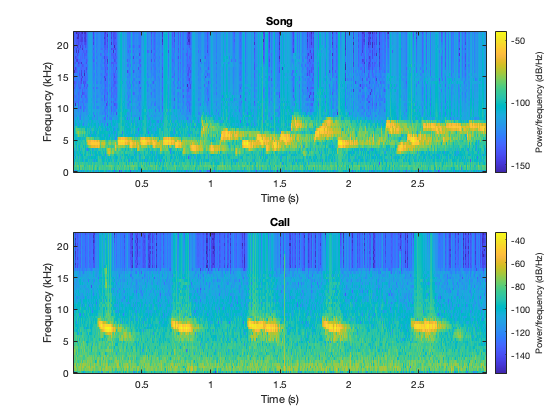
\includegraphics[width=\textwidth]{figures/wren_call_song_spectrogram.png}
  \caption{Spectrograms of the call and song of the Eurasian Wren
    (\textit{Troglodytes troglodytes}). As can be seen, the song is much more complex in terms of pitch and acoustic structure compared to the
  call}\label{fig:wren_call_song_spectrogram}
\end{figure}

Once the syllables have been segmented, there exists an abundance of options to
turn the raw syllable input signal into features that might be used as training
samples. In the following sections some of the more popular feature
representations are described, along with some novel methods that have yet to be
tried on birdsong. Note that the following list is certainly not exhaustive and
emphasis has been placed on feature representations that are relevant to this
thesis.

\subsection{Features inspired by the human auditory system}

Research has shown that birdsong and human language share many similarities in
terms of the neural mechanisms employed to form the language/song, the impact of
social contact in learning the language/song, and so on~\cite{birdsongspeech}.
Give that the human auditory system has evolved other thousands of years to best
process human speech, it seems reasonable to suggest that using features based
on the human auditory system may be effective when it comes to birdsong.

At a high level, the human auditory system works by translating changes in air
pressure originating from a source and reaching the outer ear of a listener
into vibrations that travel along an internal organ known as a cochlear. The
vibrations trigger electric signals that move along auditory nerves to the
brain, where they are interpreted as sounds. The physiology of the cochlear
means that certain parts of the organ are more sensitive to certain frequencies
of vibrations, so different frequencies will lead to different electrical
signals moving to the brain. This allows the brain to learn to differentiate
between frequencies.

\subsubsection{Mel frequency cepstrum coefficients}

The makeup of the human auditory system means that humans have a greater ability
to differentiate pitch at lower frequencies then they do at higher frequencies.
In other words, humans perceive pitch non-linearly. This has led to the
development of a logarithmic scale, known as the mel scale, such that equal
distances on the scale have the same \textit{perceptual} distance.

The mel frequency cepstrum coefficients (MFCC) are part of a family of cepstrum
coefficients that capture information about the rate of change in different
spectrum bands. MFCC differs from other cepstrum coefficients in that it uses the
mel scale to transform the spectrum of an input signal, thus utilising the human
auditory system in the calculation of its coefficients.

The $i$-th mel cepstral coefficient is computed as~\cite{davis1980comparison}
\begin{equation}
\text{MFCC}_i = \sum_{k=1}^{K} X_k \cos \left(
  \frac{i(k-0.5)\pi}{K}
\right)
\end{equation}
where $X_k$ is the logarithmic energy of the $k$-th mel-spectrum band, and $K$
is the total number of the mel-spectrum bands. Usually 8--13 MFCC coefficients
are used as the feature vector representing one time frame of the signal. The
0$^{th}$ coefficient is often excluded as it represents the average log energy
of the signal and is unlikely to carry any relevant information to help with
classification.

MFCCs are often presented with their delta ($\Delta$) and double-delta
($\Delta\Delta$) values that capture the local temporal dynamics and temporal
changes of the delta values respectively.

MFCCs are used as feature representations since they are simple to compute and
have been shown to have good performance in a wide range of audio classification
tasks, such as speaker identification~\cite{muda2010voice} and emotion
recognition~\cite{likitha2017speech}. MFCCs have also been shown to lead to good
classification accuracy for birdsong identification problems
(\cite{fagerlund2007bird} and~\cite{ramashini2022robust}).

<include graph of filterbank>

\subsubsection{Gammatone cepstrum coefficients}

Gammatone cepstrum coefficients (GTCCs) are similar to MFCCs except their
calculation  uses gammatone filterbanks instead of mel scale filterbanks.
Gammatone filterbanks are designed to simulate the motion of the membrane inside
the cochlear, known as the basilar membrane, when it is exposed to vibrations
transmitted by the outer and middle ear~\cite{patterson1992complex}.

A gammatone filter with a centre frequency $f_c$ is defined as
\begin{equation}
  g(t) = at^{n-1}e^{-2\pi b t} \cos(2\pi f_c + \psi)
\end{equation}
where $t$ is the time in seconds, $\psi$ is the phase in radians (usually set to
0), $a \in \mathbb{R}$ controls the gain, $n$ is the filter's order and $b$ is
the filter's bandwidth in Hz. To simulate the human auditory system, the centre
frequencies are uniformly spaced on the equivalent rectangular band-width (ERB)
scale.

Similar to MFCCs, GTCCs are typically used with their $\Delta$ and $\Delta\Delta$
values and have also been shown to have a good performance in
non-speech audio classification problems~\cite{valero2012gammatone}.

<include graph of filterbank>

\subsubsection{Multi resolution cochleagram}

Chen et al~\cite{chen2014feature} proposed a novel feature known as a
multi-resolution cochleagram (MRCG) that is formed by combining four
cochleagrams at different resolutions, designed to capture both local and
contextual information.

A cochleagram is formed by passing an input signal through a gammatone
filterbank, similar to the first steps of the formation of the GTCCs\@. Each
response signal from the gammatone filterbank is then divided into frames of a
certain length with a certain overlap or frame shift. The cochleagram is then
generated by calculating the power of each frame at each channel.

<example cochleagram>

A MRCG is formed by first taking one cochleagram with a frame length of 20ms and
frame shift of 10ms, using a gammatone filterbank with 64 output channels. A log
operation is applied to each time-frequency (T-F) unit of the output
cochleagram, denoted CG1. CG2 is calculated in the same way, but with a frame
length of 200ms and the same frame shift. CG3 is calculated by averaging CG1
across a square window of 11 frequency channels and 11 time frames centred at
the given T-F unit. Zero padding is used here. CG4 is calculated in the same way
as CG3, but with a $23 \times 23$ square window. CG1--4 are then stacked
vertically to obtain the full MRCG feature, which will be a $256 \times p$
matrix, where $p$ is the number of time frames.

<example mrcg>

The MRCG feature has been shown to outperform both MFCC and GTCC at
separating human speech at various SNR levels with different types of
background noise~\cite{chen2014feature}. Abdullah et
al~\cite{binti2020comparison} showed that the MRCG outperforms the Auditory
Image Model (AIM) when classifying noise. Wang et al~\cite{wang2016joint} showed
that improved speech enhancement for hearing impaired listeners was achieved
when the MRCG feature was added to the feature set.

One potential drawback when comparing the MRCG with MFCC and GTCC is the higher
dimensionality of the MRCG feature. When including the $\Delta$ and
$\Delta\Delta$ features, as is standard practice
(\cite{binti2020comparison},~\cite{wang2016joint}), the MRCG feature vector for
a single time frame has a dimensionality of 768. For MFCC or GTCC the equivalent
dimensionality is 24--39, depending on the number of the coefficients used.

\subsection{Feature stacking}

It has been shown that appropriate combining features to be used as training
inputs can lead to improved classification accuracy in audio related problems
such speech separation~\cite{wang2012exploring}. Ramashini et
al~\cite{ramashini2022robust} showed that a combination of GTCC and MFCC yielded
higher birdsong classification accuracy than MFCC alone. However, the
combination did not improve on the accuracy of GTCC alone. Yan et
al~\cite{yan2021birdsong} demonstrated that a combination of MFCC with two other
feature types (Log-mel spectrogram and Chroma) yielded higher birdsong
classification accuracy than combinations of two of the features alone.
Fagerlund~\cite{fagerlund2007bird} showed that combining MFCC with spectral and
temporal features, such as frequency range and zero crossing rate, can lead to
higher birdsong classification accuracies.

A consequence of feature stacking is that feature vectors will have increased
size. This can lead to problems such as longer training times and overfitting,
especially when used in conjunction with deep learning (DL) architectures. As a
result, dimensionality reduction techniques such as Principal Component
Analysis (PCA) or Linear Discriminant Analysis (LDA)~\cite{ramashini2019bird},
are often used to lower the dimensionality of the feature vectors while still
capturing enough information to be able to train a model effectively.

\section{Classification}

Once a suitable feature representation has been selected and performed, the
remaining task is to pick an appropriate model and train the model using the set
of training samples generated from the feature extraction.

There exist many different options in terms of models, and no one model is
superior to the others. Each problem must be considered and a model which fits
the problem at hand must be selected, or indeed a selection of suitable models
tested and the evaluated for performance.

In the literature, birdsong classification has been tackled with a wide variety
with models. Ramashini et al~\cite{ramashini2019bird} used the simple Nearest
Centroid (NC) classifier to assign birdsong samples to classes. It was compared
to a K Nearest Neighbours (KNN) classifier and shown to have superior accuracy.
Lasseck~\cite{lasseck2015improved} used decision trees with bagging to identify
birds. Trifa et al.~\cite{trifa2008automated} used Hidden Markov Models (HMM) to
identify species of birds based on their vocalizations. They considered each
sample as a discrete-time dynamical system, where an unobserved state generates
observed features, such as pitch and MFCC\@. A different HMM can be learned for
each class and a new sample can be assigned to a class by calculating which HMM
gives the highest likelihood of the observed features. Kwan et
al.~\cite{kwan2006automated} used a Gaussian Mixture Model (GMM) to classify
birds. In their experiments, a Gaussian was learned for each class of bird. A
new sample was then classified according to whichever class best describes the
new sample.

The following sections describe some models that are relevant to this thesis in
more detail

\subsection{SVMs}

SVMs are widely used in machine learning applications as a classification tool.
They are well-established due to their high accuracy
results~\cite{fagerlund2007bird} and relative simplicity to implement. Most
implementations of SVMs also require little or no tuning of hyperparameters.

At its core, a SVM is a binary classifier that separates two classes by finding
a hyperplane that maximizes the margin from the nearest vectors in the feature
space from both classes. Classifications are then made by computing in which
side of the hyperplane a test feature vector lies.

\subsubsection{Binary classification}

Let $\mathbf{x}_i \in \mathbb{R}^m$ be a feature vector of dimensionality $m$.
Let $y_i \in \left\{ +1, -1 \right\}$ be its class label. For linearly separable
data, the separating hyperplane satisfies
\begin{equation}\label{eq:svm_hyperplane}
y_i\left( \left< \mathbf{w} \cdot \mathbf{x}_i \right> + b \right) \ge 1, \hspace{1em}
i = 1,\ldots,n
\end{equation}
where $\mathbf{w} \in \mathbb{R}^m$ is a vector of weights and $b \in
\mathbb{R}$ is a bias term. The margin between the hyperplane and the nearest
feature vectors from each class is given by
\begin{align}
  \text{d}(\mathbf{w},b) &=
  \min_{\mathbf{x}_i,y_i=1}
  \frac{|\left< \mathbf{w} \cdot \mathbf{x}_i \right> + b|}{\|\mathbf{w}\|} +
  \min_{\mathbf{x}_j,y_i=-1}
  \frac{|\left< \mathbf{w} \cdot \mathbf{x}_j \right> + b|}{\|\mathbf{w}\|} \\[0.5em]
                         &= \frac{2}{\|\mathbf{w}\|}. \label{eq:svm_margin}
\end{align}

The optimal hyperplane can now be found by maximizing (\ref{eq:svm_margin})
subject to (\ref{eq:svm_hyperplane}). This can be solved using Lagrange
multipliers.

Often with real world data, classes are not linearly separable. This can
remedied by projecting the data using a nonlinear mapping into a new feature
space where the data are linearly separable. Equation (\ref{eq:svm_hyperplane})
can then be re-written as
\begin{equation}\label{eq:svm_nonlinear_mapping}
y_i\left( \left< \mathbf{w} \cdot \boldsymbol{\Phi}(\mathbf{x}_i) \right> + b \right) \ge 1, \hspace{1em}
i = 1,\ldots,n
\end{equation}
where $\boldsymbol{\Phi}$ is the nonlinear mapping. Instead of explicitly
finding $\boldsymbol{\Phi}$, (\ref{eq:svm_nonlinear_mapping}) can be re-written
in dual form
\begin{equation}
y_i\left(
  \sum_{j=1}^{l} \alpha_j y_j \left<
  \boldsymbol{\Phi}(\mathbf{x}_j) \cdot \boldsymbol{\Phi}(\mathbf{x}_i)
  \right>
\right) + b \ge 1, \hspace{1em} i=1,\ldots,n
\end{equation}
and replacing the inner product with a kernel function
$K(\mathbf{x}_j,\mathbf{x}_i) = \left< \boldsymbol{\Phi}(\mathbf{x}_j) \cdot
\boldsymbol{\Phi}(\mathbf{x}_i) \right>$.

In practice, a hyperplane that separates the classes perfectly may suffer from
poor generalization ability. To improve this, nonnegative slack variables
$\xi_i$ are introduced to (\ref{eq:svm_nonlinear_mapping}) to allow for some
missclassification of training samples in order to improve generalization
ability. The slack variables are introduced like so
\begin{equation}\label{eq:svm_nonlinear_mapping_slack}
y_i\left( \left< \mathbf{w} \cdot \boldsymbol{\Phi}(\mathbf{x}_i) \right> + b
\right) \ge 1 - \xi_i, \hspace{1em}
i = 1,\ldots,n
\end{equation}
The amount of regularization is controlled by the constant $C$ such that the
maximization problem (\ref{eq:svm_margin}) becomes
\begin{equation}
\frac{2}{\|\mathbf{w}\|} - C \sum_{i=1}^{n} \xi_i
\end{equation}

Therefore for large values of $C$ the classifier will behave like a hard-margin
SVM and attempt to perfectly classify all training samples.

The last remaining question is around what determines a valid kernel function. A
function in the input space is a kernel function if its kernel matrix
$\mathbf{K} = \left[ K(\mathbf{x}_j,\mathbf{x}_i) \right]^{n}_{i,j=1}$ is
positive semidefinite. Typical kernel functions include
\begin{itemize}

  \item linear: $K(\mathbf{x}_j,\mathbf{x}_i) = \left< \mathbf{x}_j, \mathbf{x}_i \right>$

  \item polynomial: $\left(\left< \mathbf{x}_j, \mathbf{x}_i \right> + c\right)^p$
    for some $c \in \mathbb{R}$

  \item Gaussian or RBF\@: $\exp \left( -\gamma \|\mathbf{x}_j-\mathbf{x}_i\|^2 \right)$
    for some $\gamma \in \mathbb{R}, \gamma > 0$.

\end{itemize}

\subsubsection{Multiclass classification}

SVMs can easily be extended to work with multiclass classification using
standard procedures. One procedure which is optimal with respect to the Hamming
Loss, which relates to the number of false positives or false negatives, is the
one-versus-all technique. Here, multiple SVMs are trained, each one learning the
hyperplane for samples belonging to one class versus samples belonging to all
the other classes. A new sample can then be tested against all the models and
predictions are made using the model that is most confident.

\subsection{Neural Networks}\label{ssec:nn}

Although neural networks have existed in some form since the 1950s with
inception of the perceptron algorithm~\cite{rosenblatt1958perceptron}, they have
experienced a huge surge in popularity over the past decade or so. This has
largely been due to remarkable progress being made thanks to deep neural
networks in fields such as image classification~\cite{krizhevsky2012imagenet}
and language models~\cite{mikolov2010recurrent}.

Another reason for DL's increasing popularity in recent years is due
to the availability of more performant hardware and software. The `deep' aspect
to deep learning refers to the fact that the software architecture depends on
large amounts of parameters and needs massive amounts of training data in order
to learn. In order to run training routines in a reasonable time and store large
amounts of data in memory, access to powerful hardware and/or machine
parallelism tools can be an essential part of the process.

The progress of audio problems related has also been accelerated due to deep
neural networks. Hinton et al.~\cite{hinton2012deep} showed improved performance
in speech recognition tasks using feed-forward neural networks when compared to
more classical approaches like HMMs and GMMs. Speech
enhancement~\cite{afouras2018conversation} and speech
separation~\cite{ephrat2018looking} problems leveraging DL paradigms
have also been shown to outperform more classical statistical models.

The world of birdsong classification has also benefited from DL, but
perhaps to a lesser extent than other audio related problems so far. Approaches
have mainly focused on Convolutional Neural Networks (CNNs), applying
convolutional layers to an image representation of an input signal, such as a
(Mel-)spectrogram (\cite{berger2018bird},~\cite{mukherjee2018convolutional}).
Further birdsong classification solutions have approached the problem in a
similar fashion, but utilised transfer learning to fine-tune an existing model
(\cite{disabato2021birdsong},~\cite{lasseck2018acoustic}), such as
ResNet~\cite{he2016deep} and ImageNet~\cite{deng2009imagenet}.

Disabato et al.~\cite{disabato2021birdsong} went a step further with their
research in that they considered the computational and memory demands of their
proposed bird detection DL network, ToucaNet. As mentioned earlier, DL
applications can be extremely demanding in terms of computational resources
which can make them unsuitable for running on devices with limited resources,
such as smartphones and autonomous recording units (ARUs). Their research showed
that a level of accuracy in line with the literature can be achieved but with
lower computational complexity and memory demands.

Although the architecture of DL tools for birdsong classification may vary
widely, the final layer is typically the same. This consists of a fully
connected layer of $n$ units, where $n$ is the number of classes, with a softmax
activation so that the output of the network can be considered as a probability
distribution over the classes. The softmax function is defined as
\begin{equation}
\sigma{(\mathbf{z})}_i = \frac{e^{z_i}}
  {\sum_{j=1}^{K} e^{z_j}}, \hspace{1em} i = 1,\ldots,K
\end{equation}
where $K$ is the number of classes.

A classification of an unseen sample can then be performed by assigning the
sample to the class with the highest corresponding probability.

\subsubsection{Feedforward Neural Network}

A feedforward neural network (FNN) consists of a system of connected nodes,
organised in layers, where information flows in one direction only --- forward
--- from the input nodes, through the hidden nodes (if any), and to the output
nodes. This differs fundamentally from e.g.\ a RNN, where information can flow
forward and backwards. However, both FNNs and its derivatives and RNNs share
many similarities, such as learning using backpropagation, and using nonlinear
activation functions in order to model nonlinear data.

A FNN in perhaps its most basic form while still being able to solve non-trivial
problems is known as a multilayer perceptron (MLP). An MLP consists of at least
three layers of fully connected nodes with a nonlinear activation function.
Since their inception in late 21$^{\text{st}}$ century MLPs have had extensive research
conducted into their capabilities and efficiency (\cite{hornik1989multilayer}).

<description of MLP with diagram>

MLPs have largely been superseded by more modern DL architectures such as CNN and
RNN when it comes to audio problems such as birdsong classification, however
there have been examples of more vanilla neural networks being used. McIlraith
and Card~\cite{mcilraith1997birdsong} used a two layer perceptron network using
backpropagation to minimize a mean squared error loss to classify samples from 7
birds. Murcia and Paniagua~\cite{murcia2013bird} used a simple FNN to classify
birdsong from 35 different bird species, achieving 0.74 AUC and in doing so
winning the International Conference on Machine Learning Bird Challenge 2013.

\subsubsection{Convolutional Neural Network}

CNNs have seen a huge surge in development and popularity over the last decade,
largely thanks to huge strides being made in fields like machine vision and
image classification using architectures such as
AlexNet~\cite{krizhevsky2012imagenet}. Since image and audio share many
conceptual similarities, it is reasonable to suggest that CNNs may enjoy similar
success in the world of audio classification problems. This hypothesis is
strengthened when one considers that many feature representations of audio
signals can be displayed as images, such as spectrograms
(figure~\ref{fig:wren_call_song_spectrogram}), MRCG outputs and MFCC outputs
<add links to figures here>. Indeed, there has been significant progress in
recent years thanks to CNNs in fields such as audio event
recognition~\cite{takahashi2017aenet} and automatic speech
recognition~\cite{sercu2016very}.

A CNN is a feedforward neural network with at least one convolutional layer. A
convolutional layer is so called because it performs a convolution on an input,
usually an image, using a small matrix of weights, known as a filter or kernel.
The output is considered as a matrix of activations. The activation is higher
when the values in the corresponding area in the input are similar to those in
the kernel, meaning that the activation output encodes the location of where the
input matches certain features. Usually, several kernels are applied at each
layer, and so the output takes the shape of a 3D matrix, or a volume. As with
all neural nets, the output is passed through a nonlinear activation function in
order to allow for the network to be able to learn from nonlinear data. The
weights in the kernel are learned through backpropagation. Usually a max
pooling layer is added in order to downsample the activation volume and reduce
the number of weights, or parameters, needed by the network.

<diagram of cnn>

CNNs lend themselves well to image related problems since their structure
allows them parse an image as a composition of meaningful elements rather than a
collection of unrelated pixels~\cite{lecun2015deep}. This translates well to
birdsong as e.g.\ a spectrogram of a sample of birdsong can conceptually be
thought of as a composition of syllables, i.e.\ elements.

CNNs have been applied to birdsong classification challenges with great success.
Kahl et al.~\cite{kahl2017large} achieved a remarkable mean average precision of
0.605 for a dataset of 1500 different bird species using a CNN trained on
spectrograms of 4 second samples. The spectrograms were pre-processed to reduce
noise and augmented with a variety of augmentations, such as adding Gaussian
noise and real noise samples from the original dataset. Ruff et
al.~\cite{ruff2020automated} used CNNs to detect owl vocalizations in
spectrograms from unprocessed field recordings, performing as well or better
than human experts. Narasimhan et al.~\cite{narasimhan2017simultaneous} used a
CNN with encoder-decoder architecture based on
Segnet~\cite{badrinarayanan2017segnet} to simultaneously segment and classify
birdsong spectrograms. This approach benefits from the fact that segmentation
and classification are intuitively strongly interrelated, since when comparing
two different segmentations, the one that leads to a higher classification
accuracy will likely be a better segmentation.

Ruff~\cite{ruff2020automated} looks like a good paper for this.
Kahl~\cite{kahl2017large} also.

\subsubsection{Recurrent Neural Network}

Since FNNs have a fixed size of input and output, they become unsuitable when
either the input size is variable and the output is fixed (e.g.\ with AI image
generation tools like Dall-E~\cite{ramesh2021zero}), the input size is fixed and
the output is variable (e.g.\ image captioning) or both the input size and
output size are variable (e.g.\ language translation). RNNs solve this problem
by allowing information in the network to flow in two different directions, both
forward and backward, or more precisely, in directed cycles. This is done by
feeding the output from a previous step as input to the current step, therefore
the state of the hidden units depends on the previous state of the network. This
gives the network the ability to learn long term dependencies thanks to an
unbounded previous history. The architecture of a standard RNN is shown in
figure

<figure of rnn>

Similar to FNNs, classification RNNs learn by minimizing a loss function,
usually the cross-entropy loss~\cite{shore1980axiomatic}, by backpropagation.
However, a slight variation on the algorithm is used to incorporate the
sequential nature of the input data. The variation is known as backpropagation
through time (BPTT). Here, in order to update the weights matrices, all weights
are first treated as independent. The standard backpropagation algorithm is then
run and all the corresponding gradients are averaged together. BPTT however
suffers from a problem whereby gradients larger than $\mathbf{1}$ are multiplied
together, which causes the gradient updates further back the network to
exponentially increase, which may cause memory problems. This is known as the
gradient exploding problem. The equivalent problem whereby gradients less than
$\mathbf{1}$ vanish towards 0 is known as the gradient vanishing problem. This
results in the model having no ability to learn long term dependencies. Both of
these problems are compounded by RNNs learning from long sequences of inputs,
causing longer multiplicative chains of updates. Two common approaches to
dealing with these problems is to replace vanilla RNNs with long short-term
memory (LSTM) units or gated recurrent units (GRU).

\subsubsection{LSTM}

\subsubsection{GRU}

While the usage of plain RNNs for birdsong classification has been rare in the
literature, there are several examples of birdsong classification experiments
where convolutional layers and recurrent layers have been combined to form a
Convolutional Recurrent Neural Network (CRNN)
(\cite{yan2021birdsong},~\cite{mukherjee2018convolutional}) in order to leverage
the benefits of both architectures. A typical approach using a CRNN with regards
to birdsong classification might look something like the
following~\cite{crous2019polyphonic}

\begin{enumerate}

  \item Convert an audio segment to a frequency domain representation to be
    interpreted as an image, e.g.\ a spectrogram.

  \item Apply a convolutional layer (or layers) to each time step of the
    representation in order to extract local features. A time step is defined as
    a single unit along the time axis of the spectrogram.

  \item Apply a recurrent layer to spread the local features of a single time
    step to its temporal surroundings. The spread features can then be processed
    by a fully connected layer with softmax activation as described in
    Section~\ref{ssec:nn} to make a prediction in the form of a distribution
    over output classes for each time step.

\end{enumerate}

The recurrent layer provides two key advantages compared to a plain CNN\@.
Firstly, the network will be able to learn from previous and future features in
order to strengthen predictions. For example, if the current time step equally
supports a blackbird or a nightingale prediction by itself, it will be skewed
towards a blackbird if the previous time step and future time step both
predicted a blackbird. Secondly, the network can learn to include moments of
silence in a prediction. Note that this benefit is lost if just considering
audio segments of isolated syllables as these segments should contain little or
no silence.

Check refs in the Narasimhan paper~\cite{narasimhan2017simultaneous}.


\chapter{Methodology}
Describe your method in detail and with great clarity, distinguishing it from
other works (if it is indeed a novel idea). It is very important to clearly
motivate your method.

Describe the results of your method here in this chapter.

All computational work for this thesis was performed in \textit{MATLAB vR2023a}
unless stated otherwise.

\section{Datasets}

Crous~\cite{crous2019polyphonic} has some data on Xeno-canto.

Since all the models described in Section~\ref{sec:classification} are trained
in a supervised learning fashion, this requires a dataset of labelled training
examples. The website xeno-canto.org (XC) houses the largest and most
comprehensive publicly available collection of birdsong samples in the world. It
has made an enormous impact in the field birdsong recognition since its
inception in 2005 and has been source of the datasets for the annual BirdCLEF
challenge since 2014~\cite{vellinga2015xeno}. All samples available on XC are
labelled with the bird species and contain rich metadata, such as the time and
location of the recording. Importantly, all samples have a crowd-sourced rating
from A --- E which signifies how clear the recording sample is, where A denotes
samples with the highest quality and clarity. This is especially important
should we wish to experiment with different signal-to-noise ratios (SNR) as the
noise can be manually added to a clean recording at precise SNR levels.

Due to its scale and reputation in the birdsong classification community, all
samples used in this thesis have been downloaded from the XC repository. All
samples downloaded have an A rating and have been labelled as a `song' rather
than a `call'. The samples are stored in a directory labelled according to the
first three letter of species' binomial name. For example, samples from the
common blackbird (\textit{Turdus merula}) are stored in a directory called
`TURMER'. This directory name acts as a label for training and test samples.

In this work we are mostly concerned with testing relative improvements in model
performance after tuning various components, such as novel feature
representations. To this end, we select the most simple form of classification
experiment: binary classification. The two bird classes selected for all
experiments herein are the common blackbird and the common nightingale
(\textit{Luscinia megarhynchos}) due to the two birds' vocalizations being
acoustically similar and hence more difficult to distinguish resulting in more
variable accuracy results, and the author's personal preference.

Roughly 38 individuals from each class were downloaded, with 28 used for
training and the remaining kept for testing.

\section{Pre-processing}

Some recordings available on XC are recorded in stereo sound, so in order to
reduce dimensionality without losing too much information, all stereo recordings
are first converted to mono by taking a mean average of both channels. Leading
and trailing sections of background noise are then stripped from the recording
using the \textit{detectSpeech} function provided by \textit{MATLAB}. This
function uses a thresholding algorithm to detect onset and offset indices of
speech~\cite{giannakopoulos2009method}. The function works for birdsong since
birdsong frequencies reside in a similar range to that of human speech. The
function accepts various arguments to determine properties such as window length
and threshold value, but from initial experiments the function was shown to
work well with birdsong with the defaults, see figure~\ref{fig:detected_speech}.
The detected onset and offset of birdsong allows for the leading and trailing
bits of background noise to be removed from the recording, thus reducing
unnecessary computational time in segmenting the audio.

\begin{figure}[ht]
  \centering
  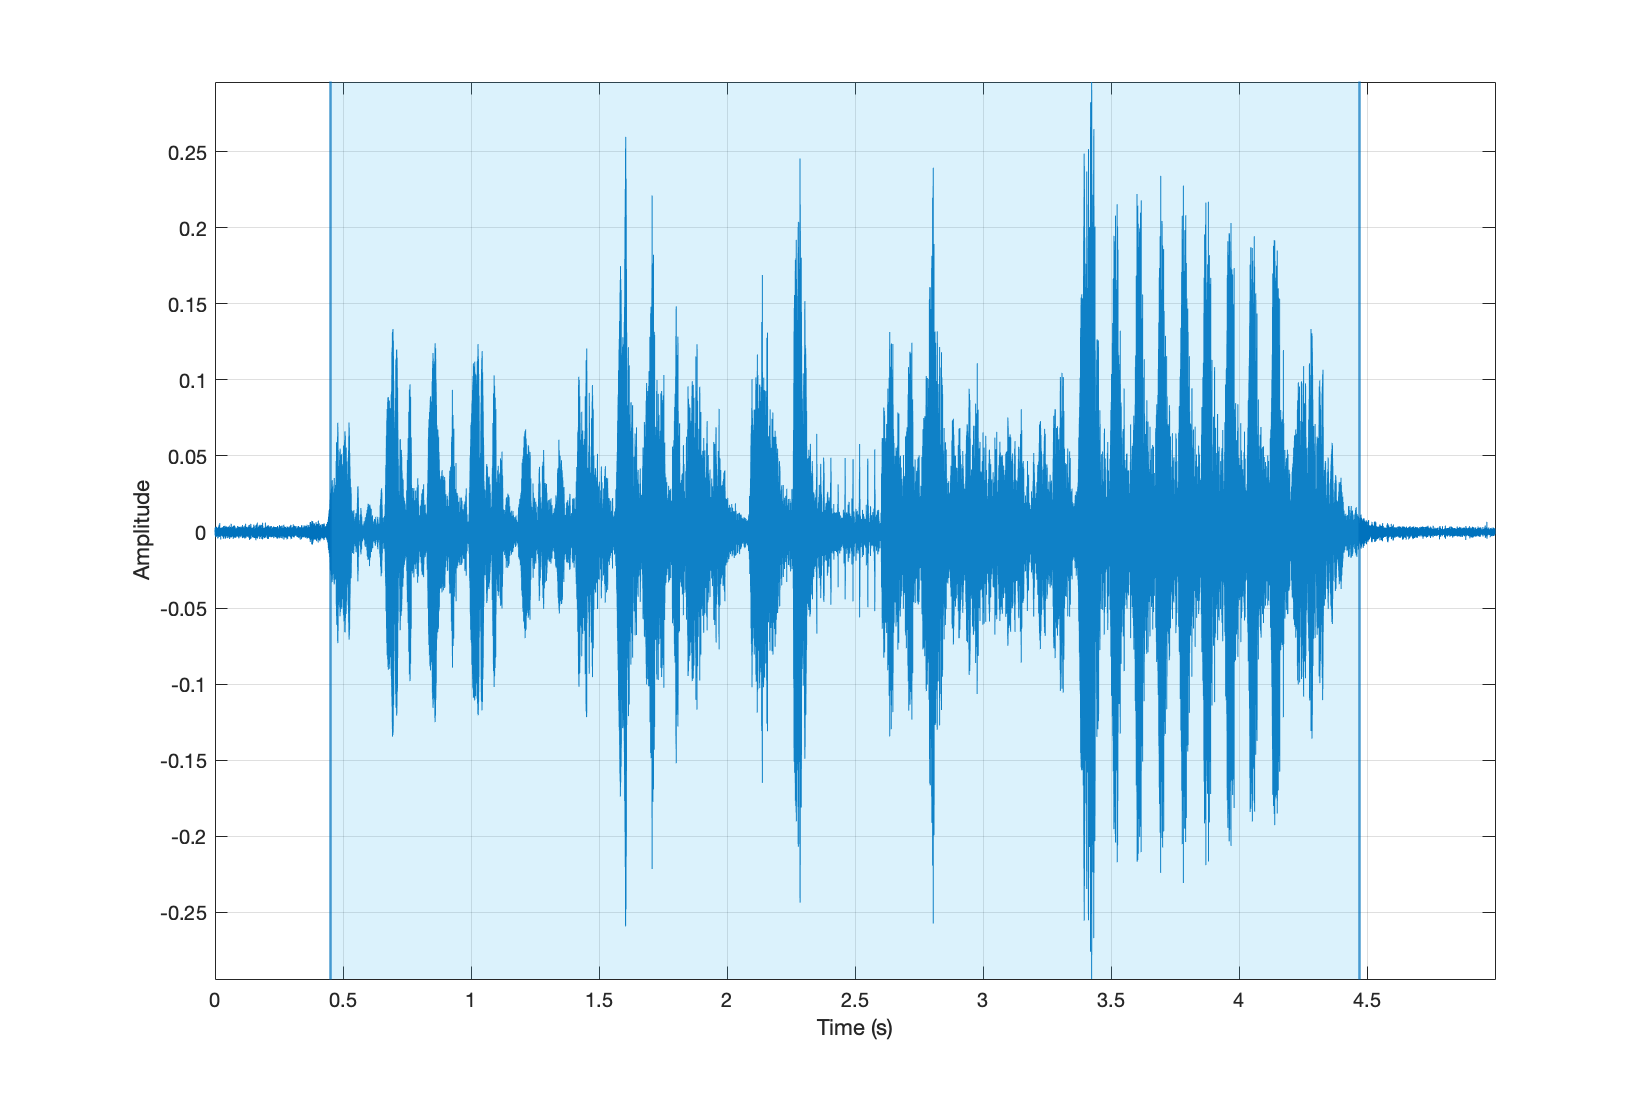
\includegraphics[width=\textwidth]{figures/detected_speech.png}
  \caption{Output of the \textit{detectSpeech} function for a recording of
  birdsong from a Eurasian wren. The highlighted section shows where the
algorithm has detected `speech', or in this case,
birdsong.}\label{fig:detected_speech}
\end{figure}

A highpass filter is then applied to the recording with a passband frequency of
450Hz. This value was chosen as most birdsong sits in the range of 1KHz ---
10Khz, and so lower frequencies can be attributed to background noise and
therefore their removal should reduce noise in the system without losing
important information. The reason why frequencies above 10Khz are not removed
is that, as can be seen from figure~\ref{fig:wren_call_song_spectrogram}, birds
typically produce higher frequency harmonics when vocalizing, shown as vertical
bands moving upwards from where syllables are located on the spectrogram. These
harmonics may capture useful information for the learning algorithm to utilise
and should therefore not be filtered out.

After these pre-processing steps have been taken, the audio is ready for
syllable segmentation.

\section{Segmentation}\label{sec:segmentation}

Recordings downloaded from XC were also chosen based on their length. Recordings
of duration 40 seconds to 120 seconds were preferred since they were likely to
be long enough to include enough variety of vocalizations from one individual
bird, but not too long so as to take up too much space on disk. In this thesis
it was preferred to have fewer samples from more individual as opposed to more
samples from fewer individuals for each species. The intention of this was to
introduce more variation in the training samples for each class, especially when
considering that many birds of the same species but residing in different
locations have demonstrated subtle variations in vocalizations, known as
dialects~\cite{baker1985biology}. As a general rule of thumb, a target of
roughly 50 training samples per individual was aimed for in this thesis.

This leads to the question of how to generate samples. In the literature there
seem to be two main ways of segmenting recordings into samples to be used for
training. The first is segmenting a recording into overlapping segments of a
certain length, typically in the range of 4 --- 11 seconds
(\cite{yan2021birdsong},~\cite{crous2019polyphonic}). This has the advantage
that all samples will be of fixed length and that the segmentation algorithm is
very simple. However, it will likely mean that some samples will contain only
background noise which, if used for training, will introduce noise into the
system. These noise samples therefore may need to be removed, either
manually~\cite{yan2021birdsong} or using an
algorithm~\cite{narasimhan2017simultaneous}. The other method involves
segmenting the recording into syllables
(\cite{fagerlund2007bird},~\cite{ramashini2022robust}). This has the advantage
that all training samples are likely to contain little or no noise. However the
samples will be of variable length, so steps will be needed to be taken in order
to compare the samples, such as adding padding or more advanced techniques like
dynamic time warping~\cite{somervuo2006parametric}. Syllable segmentation also
has the enticing prospect of being able to identify a bird species from a very
short sample. This could be useful in situations where a recording is mostly
corrupted by background noise but has a few small segments of clear birdsong.

In this work we attempt to combine the benefits of both approaches by first
segmenting a recording to retrieve the syllables using a process described in
Section~\ref{ssec:syllable_seg}. Then, for each syllable, the
following syllables are appended until a fixed sample length is reached. If a
syllable is added which pushes the sample length over the limit, then the sample
is trimmed at the fixed length. This approach is motivated by Somervuo et al.'s
work~\cite{somervuo2006parametric} in showing that training and classifying
using single syllables returns suboptimal results, whereas using sequences of
syllables gives much improved accuracy. Of course there is a tradeoff here
between training with longer sequences, and hence more information, versus
increased computational demand to perform training.

\begin{figure}[ht]
  \centering
  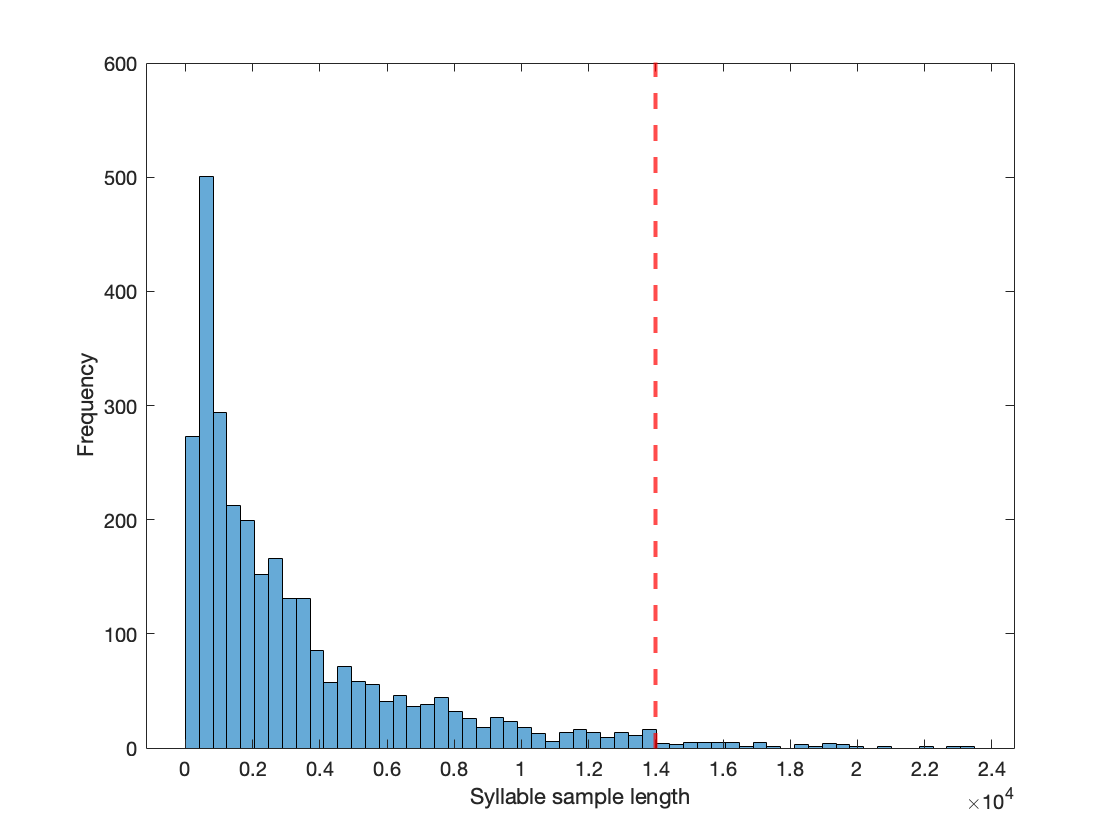
\includegraphics[width=\textwidth]{figures/syllable_sample_length.png}
  \caption{Histogram showing the frequency of different sample lengths for all
  training syllables. A candidate fixed sequence length is denoted by the red
dashed line.}\label{fig:syllable_sample_lengths}
\end{figure}

From figure~\ref{fig:syllable_sample_lengths}, we can see most syllable lengths
fall in the region $\left[ 200, 1236 \right]$ (the segmentation algorithm sets a
minimum of 200 samples for candidate syllables). Therefore a sequence of fixed
length about 14000 (denoted by the red dashed line) should contain between 10
and 70 syllables. The fixed length, equating to about 3ms duration, also ensures
that most sequences contain at least one full syllable. This approach ensures
the influence of background noise is kept to a minimum, while still maintaining
information related to the temporal evolution of a particular birdsong.

\subsection{Energy based syllable segmentation}\label{ssec:syllable_seg}

This algorithm was first proposed by Fagerlund~\cite{fagerlund2004automatic}
and has been used in various research papers since
(\cite{somervuo2006parametric},~\cite{ramashini2022robust}). Note that Fagerlund
proposed two different segmentation methods in the paper. In this thesis we use
the energy based segmentation method as it's relatively
simple to implement and its performance can be superior to the other method
proposed. The algorithm is computed in the following 3 phases:

\begin{enumerate}

  \item Determine the onsets and offsets of syllable candidates. Special
    attention has to be paid to the border effect~\cite{li2001classification},
    whereby the energy envelope near onsets and offsets fluctuates around a
    threshold.

  \item Syllable candidates that are within a certain temporal distance with
    each other are merged into one. The initial separation of candidates can
    likely be attributed to the border effect, and so the candidates can be
    thought of as originating from one syllable in reality.

  \item Syllable candidates that are shorter than a minimum threshold are
    removed. These candidates are often caused by random fluctuations in the
    signal energy and are unrelated to bird vocalizations.

\end{enumerate}

\subsubsection{Onset/offset detection}

The first phase considers the energy of an input signal. The energy envelope is
the key variable to use in determining the onset and offset of a syllable. The
general idea is that when the energy increases past a threshold, this marks the
start of a syllable candidate and when the energy then falls below the same
threshold, this marks the end of a syllable candidate. To calculate the energy
envelope, the recording is divided into overlapping frames.
Fagerlund~\cite{fagerlund2004automatic} recommends a frame size of 128 samples
and an overlap of 50\%. This corresponds to a frame length of roughly 3ms. Since
distance between syllables can be as short as 20ms, the frame size needs to be
small enough so that there are at least a few frames between candidates to be
able to efficiently discriminate between syllables.

Frames are first windowed using a Hanning window. The energy $E_i$ in the
decibel scale for frame $i$ is calculated as
\begin{equation}
  E_i = 10 \log_{10} \sum_{j=1}^{K} x{(i)}_{j}^2
\end{equation}
where $x{(i)}_j$ is the $j^{\text{th}}$ input signal sample value in the
$i^{\text{th}}$ frame and $K$ is the total number of samples in each frame, in
this case 128. The maximum energy of the entire signal is normalized to 0dB. The
initial noise level estimate is set to be equal to global minimum value of the
energy envelope and the threshold for the onset and offset detection is set to
half the noise estimate. The flow diagram for onset and offset detection can be
seen in figure <figure of flow chart>. In essence, the algorithm moves through
each frame and computes whether the frame should be assigned to a syllable or
not, updating noise and energy thresholds as it goes. The noise estimate is
updated as the average energy of frames already processed by the algorithm that
are not assigned to a syllable.

\subsubsection{Merging syllable candidates}

The algorithm may produce syllable candidates that are very temporally close
together. This may be from the bird producing short bursts of pulses that
constitute the same syllable, or it may be from the border effect. In both cases
the candidates can be considered as belonging to the same syllable and so can be
safely merged together. Candidates that are less than 15ms apart are selected
for merging~\cite{fagerlund2004automatic}.

<figures of segmentation>

Each segmented syllable is then stored as an individual \textit{wav} file in the
same directory as the original recording with a filename in the format
\textit{\{XCID\}\_i.wav} where \textit{XCID} is the XC id of the recording and
\textit{i} is the index of the syllable.

\section{Feature extraction}

Once syllables have been extracted and stored as individual audio files, they
are ready to be retrieved and converted to features. As mentioned in
Section~\ref{sec:segmentation}, before feature extraction is performed,
syllables are concatenated together until a minimum length is achieved.

\subsection{Cepstral coefficients}

The cepstral coefficients on which this thesis focuses are the MFCC and GTCC\@.
Both features are extracted using builtin \textit{MATLAB} functions
\textit{mfcc} and \textit{gtcc} respectively. The functions accept arguments
which affect how the routine processes input signals. To the best of the
author's knowledge, these arguments have not been explored in the field of
birdsong classification problems.

\subsubsection{MFCC}\label{sssec:mfcc}

A potentially overlooked parameter of MFCC extraction with regards to birdsong
classification using \textit{MATLAB} is the \textit{BandEdges} argument. This
argument provides the basis of the half-overlapped triangular filters that
\textit{mfcc} uses. By default, \textit{BandEdges} is a 42-element vector that
results in a 40-band filter bank constructed using 13 linearly-spaced filters,
with 133.3Hz separating their center frequencies, and 27 log-spaced filters,
separated by a factor of 1.0711703 in frequency~\cite{slaney1998auditory}. This
equates to a frequency range that spans approximately 133Hz to 6864Hz. This
range is well suited to human speech, of which MFCC is often used as a feature,
but may be less suitable for birdsong which can sometimes sit outside the normal
frequency range of human speech.

In this work we consider alternative constructions of the MFCC filter banks,
such as extending the range and adding more filters and assess the performance
of classifiers using the alternative MFCC filter banks in comparison with the
default.

\subsubsection{GTCC}\label{sssec:gtcc}

Like MFCC, GTCC has a potentially overlooked argument in
\textit{FrequencyRange}. This two-element row vector specifies the minimum and
maximum values in Hz of the gammatone filter bank used by the \textit{gtcc}
routine. The default value is \texttt{[50, fs/2]}, which could potentially be
fine-tuned for birdsong related problems since birdsong frequencies do not
typically go below 1Khz.

In this work we consider alternative values for the maximum and minimum
frequency of the gammatone filter bank and compare performance of classifiers
trained using the alternative GTCC representations with the default.

\subsection{MRCG}

\textit{MATLAB} provides no builtin functions for computing an MRCG, or even a
cochleagram, upon which the MRCG is based. To that end, custom code was
developed based on the toolbox developed by Kim and Hahn~\cite{kim2018voice}
which implements MRCG\@. The MRCG routine implemented in~\cite{kim2018voice}
uses a gammatone filter bank with a frequency range of \texttt{[50, 8000]},
which may not be suitable for birdsong problems. The work done in customising
the toolbox for this thesis extends the implementation to work with alternative
frequency ranges for the gammatone filter bank.

It's recommended to include the $\Delta$ and $\Delta\Delta$ values along with
the MRCG feature~\cite{chen2014feature}, so hereafter the term MRCG shall refer to
the base MRCG along with its $\Delta$ and $\Delta\Delta$ values. The same
applies to MFCC and GTCC\@.

Due to the high dimensionality of the MRCG feature and considering the
computational limitations of the machine upon which the training for this thesis
was performed, the MRCG feature would be best suited to a classifier which is
optimised for working with image data, such as CNNs\@. To that end, it won't
be used with SVMs in this work.

\section{Training}\label{sec:training}

To create the training cell array, syllables are retrieved and concatenated to form
a training sample, hereafter referred to as a sequence. A maximum limit of 40
sequences per individual is imposed to ensure enough variation while keeping
training times to a minimum. The number of training sequences used for both
classes can be seen in table~\ref{table:training_samples}.

\begin{table}[h!t]
\begin{center}
\begin{tabular}{c c c}
\toprule
Class & Individuals & Sequences \\ [0.5ex]
\midrule
Common blackbird (\textit{TURMER}) & 28 & 1107 \\
Common nightingale (\textit{LUSMEG}) & 28 & 1200 \\
\bottomrule
\end{tabular}
\caption{Number of training sequences for used for both
classes.}\label{table:training_samples}
\end{center}
\end{table}

The training cell is formed by vertically concatenating the two cell arrays
containing the training sequences to form a $2311 \times 1$ cell array. The
training labels are contained in a $2311 \times 1$ categorical array with a
\textit{TURMER} category labelling a blackbird sequence and \textit{LUSMEG}
labelling a nightingale sequence.

All training is performed on an Apple MacBook Pro (late 2013) running OSX
11.5.2.

\subsection{SVMs}

All SVM models are implemented using \textit{MATLAB's} \texttt{fitcsvm}
function provided in the Statistics and Machine Learning Toolbox.

SVMs require each training sample to be a row vector. To convert the training
cell array to the required matrix format, a function can be applied to each cell
using the \texttt{cellfun} function to extract the desired feature and flatten
the output to a row vector. A simple routine can then be applied to convert the
cell array to a matrix of numerical data, the required format for
\texttt{fitcsvm}. The training labels cell array mentioned in the previous
section requires no transformation.

\subsubsection{Linear}

Linear SVMs are trained by supplying a \textit{KernelFunction} argument set to
\textit{linear} to the \texttt{fitcsvm} function. Linear SVMs are reasonably
simple to fit as they have fewer parameters than SVMs utilising other kernel
functions. The key parameter to tune for here is the \textit{BoxConstraint},
which controls the trade-off between maximizing the margin between classes and
minimizing the classification error. This is the constant $C$ in Equation
(\ref{eq:svm_nonlinear_mapping_slack}). The \textit{Standardize} parameter
controls whether data is standardized before fitting, and can also affect the
performance of the model. In this work, KFold cross-validation (KF) was selected
to optimize the parameters, with $K=7$ folds. This is motivated by other
research taking the same approach with promising
results~\cite{ramashini2022robust}.

Figure~\ref{fig:linear_optim} shows where the optimum values of
\textit{BoxConstraint} and \textit{Standardize} lie for a linear SVM\@. As can
be seen, the \textit{Standardize} parameter makes a slight difference on model
performance, whereas \textit{BoxConstraint} makes a significant difference, with
lower values preferred. A lower value means that the model has greater
flexibility in misclassifying training samples for the benefit of better
generalization.

\begin{figure}[ht]
  \centering
  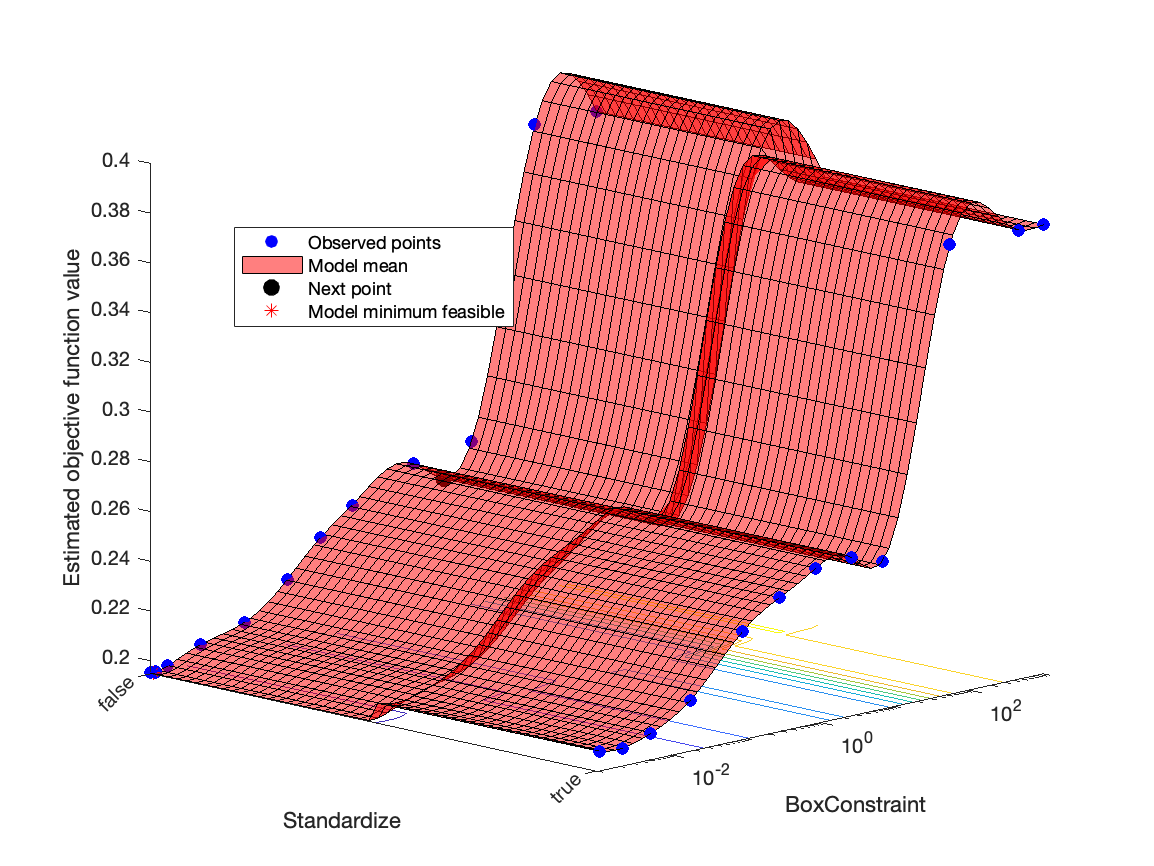
\includegraphics[width=\textwidth]{figures/linear_optim.png}
  \caption{Plot showing optimum values of the \textit{BoxConstraint} and
  \textit{Standardize} parameters when fitting a linear SVM.\ The optimum values
are located where the objective function is at a
minimum.}\label{fig:linear_optim}
\end{figure}

\subsubsection{RBF}

RBF SVMs are able to fit more complex decision boundaries by projecting data
into a higher dimensional space, which is controlled by the hyperparameter
\textit{KernelScale}. RBF SVMs are also sensitive to the \textit{BoxConstraint}
parameter. 7-fold cross validation was performed using a \texttt{cvpartition}
and supplying a \textit{OptimizeHyperparameters} argument set to \textit{auto}
to \texttt{fitcsvm}. A value of \textit{auto} means that both
\textit{KernelScale} and \textit{BoxConstraint} are optimised during training.

Figure~\ref{fig:rbf_optim} shows where the optimum values of
\textit{BoxConstraint} and \textit{KernelScale} lie for a RBF SVM\@. Both
parameters are shown to have an impact on the model performance, with high
values of \textit{BoxConstraint} and mid-range values of \textit{KernelScale}
preferred. <what does kernel scale do?>

\begin{figure}[ht]
  \centering
  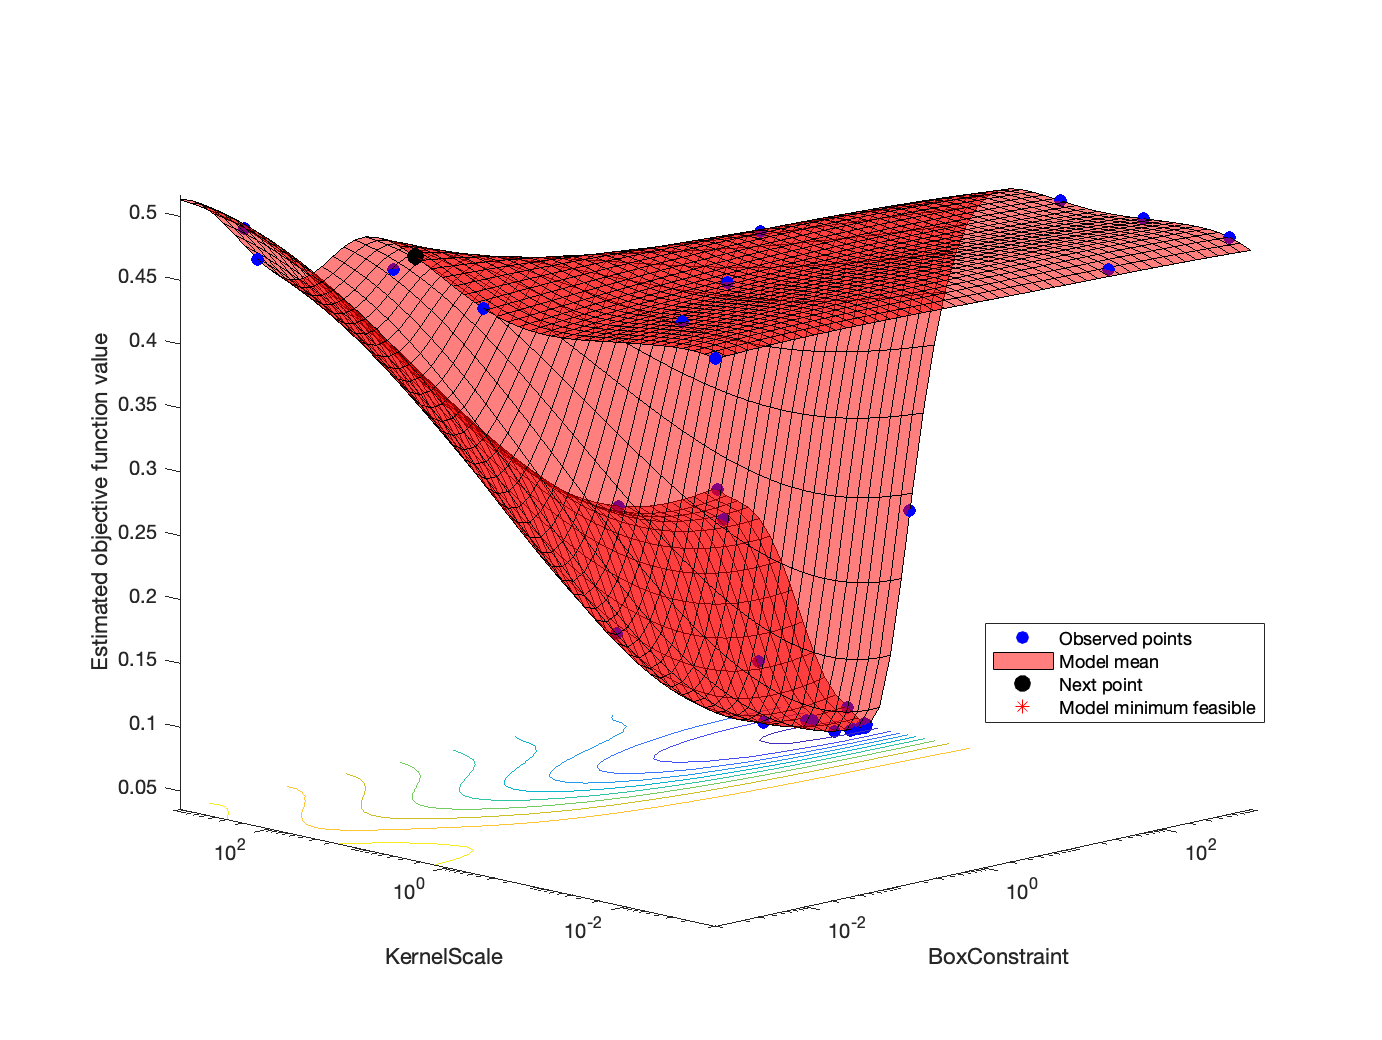
\includegraphics[width=\textwidth]{figures/rbf_optim.png}
  \caption{Plot showing optimum values of the \textit{BoxConstraint} and
  \textit{KernelScale} parameters when fitting a RBF SVM.\ The optimum values
are located where the objective function is at a
minimum.}\label{fig:rbf_optim}
\end{figure}

\subsection{Neural networks}

\section{Evaluation}

After the recordings from each class reserved for testing have undergone
pre-processing and segmentation, the segmented syllables undergo the same
routine described in Section~\ref{sec:training} to generate the testing
sequences. The number of testing sequences used for both classes can be seen in
table~\ref{table:testing_samples}.

\begin{table}[h!t]
\begin{center}
\begin{tabular}{c c c}
\toprule
Class & Individuals & Sequences \\ [0.5ex]
\midrule
Common blackbird (\textit{TURMER}) & 9 & 360 \\
Common nightingale (\textit{LUSMEG}) & 10 & 400 \\
\bottomrule
\end{tabular}
\caption{Number of testing sequences for used for both
classes.}\label{table:testing_samples}
\end{center}
\end{table}

A testing cell is created in the same way as the training cell and is used for
evaluating all models in this thesis.

\subsection{AUC}

As mentioned in Section~\ref{sec:eval_metrics}, the AUC metric is commonly used
for binary classification problems, and has been frequently used as a metric in
birdsong classification problems. Further to the advantages listed in 
previously, the AUC benefits from being unaffected from class imbalances.
Although the positive and negative classes are only slightly imbalanced in this
work (see Table~\ref{table:training_samples}), it makes sense to use a metric
that is unaffected by class imbalance all the same.

The AUC is calculated using the \texttt{perfcurve} function which checks the
class prediction scores returned by the model against the true labels.

\subsection{Classification accuracy}

Since the classes are only slightly imbalanced, the classification accuracy
provides a reasonably unbiased, quick, and easily interpretable snapshot at how
well a model has performed. It is calculated as
\begin{equation}
A = \frac{1}{N}\sum_{i=1}^{N} \mathbb{I}[\bar{y}_i = y_i]
\end{equation}
where $N$ is the number of test samples, $\bar{y}$ is a predicted label, $y$
is the groundtruth label, and $\mathbb{I}$ is the indicator function.

\section{Extensions of methodology}


\chapter{Results \& Discussion}
\section{Hypothesis 1}

Hypothesis 1 (H1) is stated as follows:

\begin{quote}
Explore some of the hyperparameters available during the feature extraction
process. The hypothesis is that using hyperparameter values more suited to
birdsong classification problems will yield a higher classification accuracy.
\end{quote}

H1 was applied to two feature extraction processes that appear in some form
widely in the literature related to birdsong classification: MFCC and GTCC\@.

\subsection{MFCC}

The key parameter under test in this work as mentioned in
Section~\ref{sssec:mfcc} is the \textit{BandEdges} argument. 7 experiments were
devised and evaluated in order to see if any improvements to binary bird
classification models utilising MFCC could be made with adjusted
\textit{BandEdges} arguments. The experiments are listed in
Table~\ref{table:h1_mfcc_experiments}.

\begin{table}[h!t]
\begin{center}
\begin{tabular}{c c c c}
\toprule
Number & Number of bands & Band type & Approximate frequency range (Hz) \\ [0.5ex]
\midrule
1 & 40 & Mel & 133 --- 6864 \\
2 & 40 & Mel & 50 --- $\text{fs}/2$ \\
3 & 80 & Mel & 50 --- $\text{fs}/2$ \\
4 & 40 & Linear & 50 --- $\text{fs}/2$ \\
5 & 40 & Linear & 133 --- 6864 \\
6 & 40 & A-mel & 133 --- 6864 \\
7 & 40 & Mel & 133 --- 10000 \\
\bottomrule
\end{tabular}
\caption{Description of experiments used for testing H1 with
MFCC.}\label{table:h1_mfcc_experiments}
\end{center}
\end{table}

\subsubsection{Comments on experiment setup}

In the table, `fs' refers to the frequency sampling rate for a given audio file,
usually 44.1 KHz or 48 KHz. $\text{fs}/2$ is the maximum possible value for the
\textit{BandEdges} argument. `A-mel', short for anti-mel, denotes a set of mel
filterbanks that have been inverted, such that the center frequencies are closer
together at higher frequencies and further apart at lower frequencies. `Linear'
refers to a set of filterbanks that have been spaced linearly on the frequency
scale. The different band types can be visualized in figure

<figure of the different band types>

The experiment design was motivated as follows:

\begin{itemize}

  \item [Exp 1:] These are the defaults provided with the \texttt{mfcc}
    function and acts as a control experiment.

  \item [Exp 2:] A wider frequency range may be able to make use of the
    higher frequency harmonics produced by most birdsong.

  \item [Exp 3:] A wider frequency range means the bands have a larger bandwidth
    and may lose some distinguishing power. Increasing the number of bands may
    help to alleviate this.

  \item [Exp 4:] Since the human auditory system hasn't evolved specifically to be
    able to distinguish birdsong, it's entirely possible that the mel scale
    isn't the optimum scale to use. A linearly spaced set of filterbanks may
    provide a good generalised attempt at distinguishing birdsong.

  \item [Exp 5:] Similar to Experiment 4 but focused on a frequency range that
    more tightly fits around the dominant frequencies produced by bird
    vocalizations.

  \item [Exp 6:] The anti-mel scale has been used with interesting results in
    human speech recognition through telephones~\cite{lei2009mel}. It offers
    more distinguishing power at higher frequencies, and since birdsong is
    typically produced at higher frequencies than human speech, the anti-mel
    scale may be able to better distinguish birdsong.

  \item [Exp 7:] Similar to Experiment 2 but still focused on the main
    frequencies emitted by birds.

\end{itemize}

\subsubsection{Results}

A chart of both the AUC and the classification accuracy for MFCC can be seen in
figure~\ref{fig:hyp1_mfcc}.

\begin{figure}[ht]
  \centering
  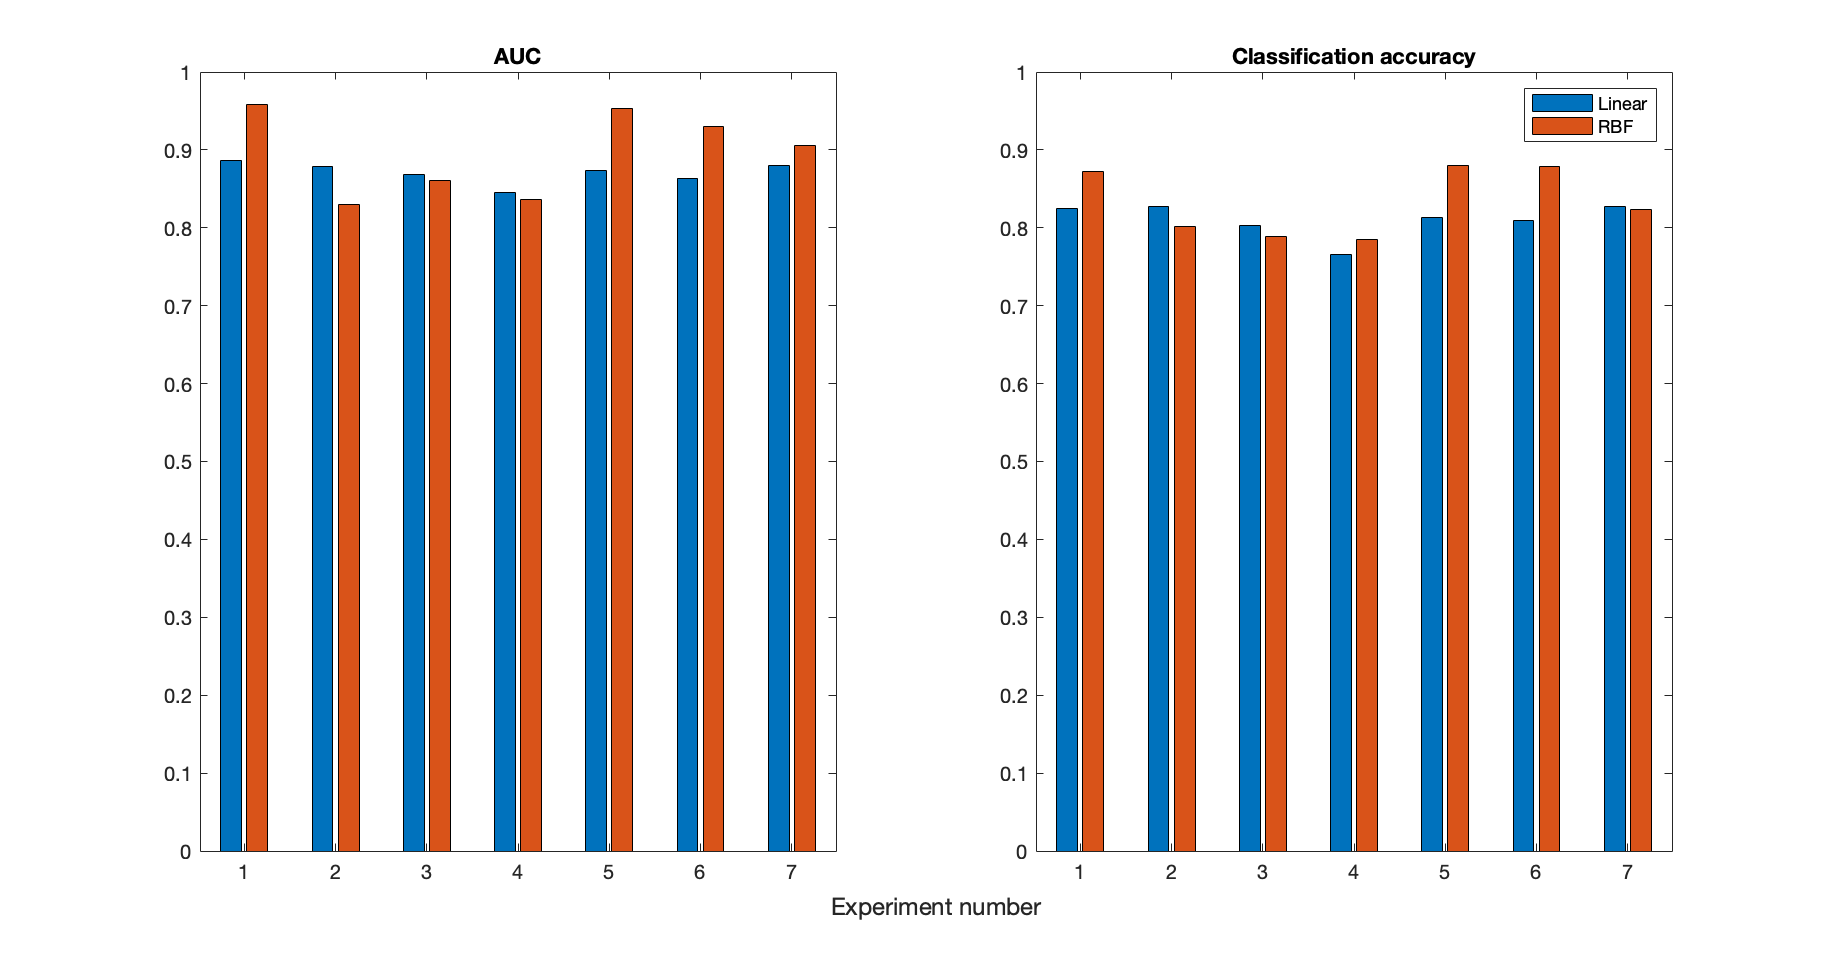
\includegraphics[width=\textwidth]{figures/hyp1_mfcc.png}
  \caption{The AUC and classification accuracy scores for linear and RBF models
  for different experiments for MFCC.}\label{fig:hyp1_mfcc}
\end{figure}

As shown in the chart, both evaluation metrics are highest in the control
experiment. Experiment 5 returns comparable metrics to the control experiment,
with slight improvements made to the classification accuracy for the RBF model.
The RBF model shows a clear reduction in performance for wider frequency ranges
across both evaluation metrics.


\chapter{Conclusion}
In this work we have thoroughly investigated some important parameters when
extracting classic features like MFCC and GTCC\@. We have shown that the
parameters can have a significant effect on the overall classification accuracy
and that the parameter values should be carefully considered for the problem at
hand. During this investigation we have shown that MFCC usually outperforms GTCC
when the sample recordings are clean.

We have also investigated some more complex and modern architectures such as CNN
and RNN and have confirmed that they can easily outperform more classical models
like SVM\@. In doing so we have also proposed a novel method of generating
training and testing samples by combining syllables, the elemental blocks of
birdsong. We have also laid the theoretical groundwork for an alternative form
of sample generation that can be used with CRNN in future work.

The main contribution of this study is the application of MRCG to birdsong
classification. While the results achieved here were less than desirable, it's
unclear whether this is from the model design or the suitability of MRCG with
birdsong as some concessions had to be made to allow for MRCG's significantly
higher dimensionality compared to classic features such as MFCC\@. This could be
verified by testing MRCG with some more complex CNN or CRNN model architectures
on more powerful machines.


\appendix

\bibliographystyle{plain}
\bibliography{refs}

\end{document}
